\documentclass[12pt,a4paper]{article}
\usepackage[utf8]{inputenc}
\usepackage[german]{babel}
\usepackage[T1]{fontenc}
\usepackage{amsmath}
\usepackage{amsfonts}
\usepackage{amssymb}
\usepackage{graphicx}
\usepackage[left=2.5cm,right=2.5cm,top=2cm,bottom=2cm]{geometry}
\usepackage{float}
\author{Gruppe C14 \\ Julián Häck, Martin Koytek, Lars Wenning, Erik Zimmermann}
\begin{document}
\section{Stimmen der Gitarre über Schwebung}
\subsection{Versuchsbeschreibung}
Schlägt man an einer Gitarre 2 Saiten so an, dass sie denselben Ton erzeugen ergibt sich, wenn die Töne nur leicht voneinander abweichen, eine Schwebung. Nur wenn die Töne exakt gleich sind verschwindet die Schwebung. \newline
In diesem Versuch sollte eine Saite einer Gitarre mit Hilfe der Schwebung gestimmt werden.
\subsection{Versuchsaufbau und Durchführung}

Zu aller erst wurden alle Saiten der Gitarre mit einem Stimmgerät gestimmt.  \newline
Daraufhin wurde die Gitarre auf den Tisch gelegt und die Frequenz jeweils mit einem Mikrofon, das über dem Schallloch der Gitarre angebracht war, aufgenommen. Das Signal des Mikrofons wurde mit dem Spannungsmessgerät des Sensor-Cassy vermessen, um schließlich mit Cassy-Lab am Laptop ausgewertet werden zu können.

\begin{figure}[H]
\centering
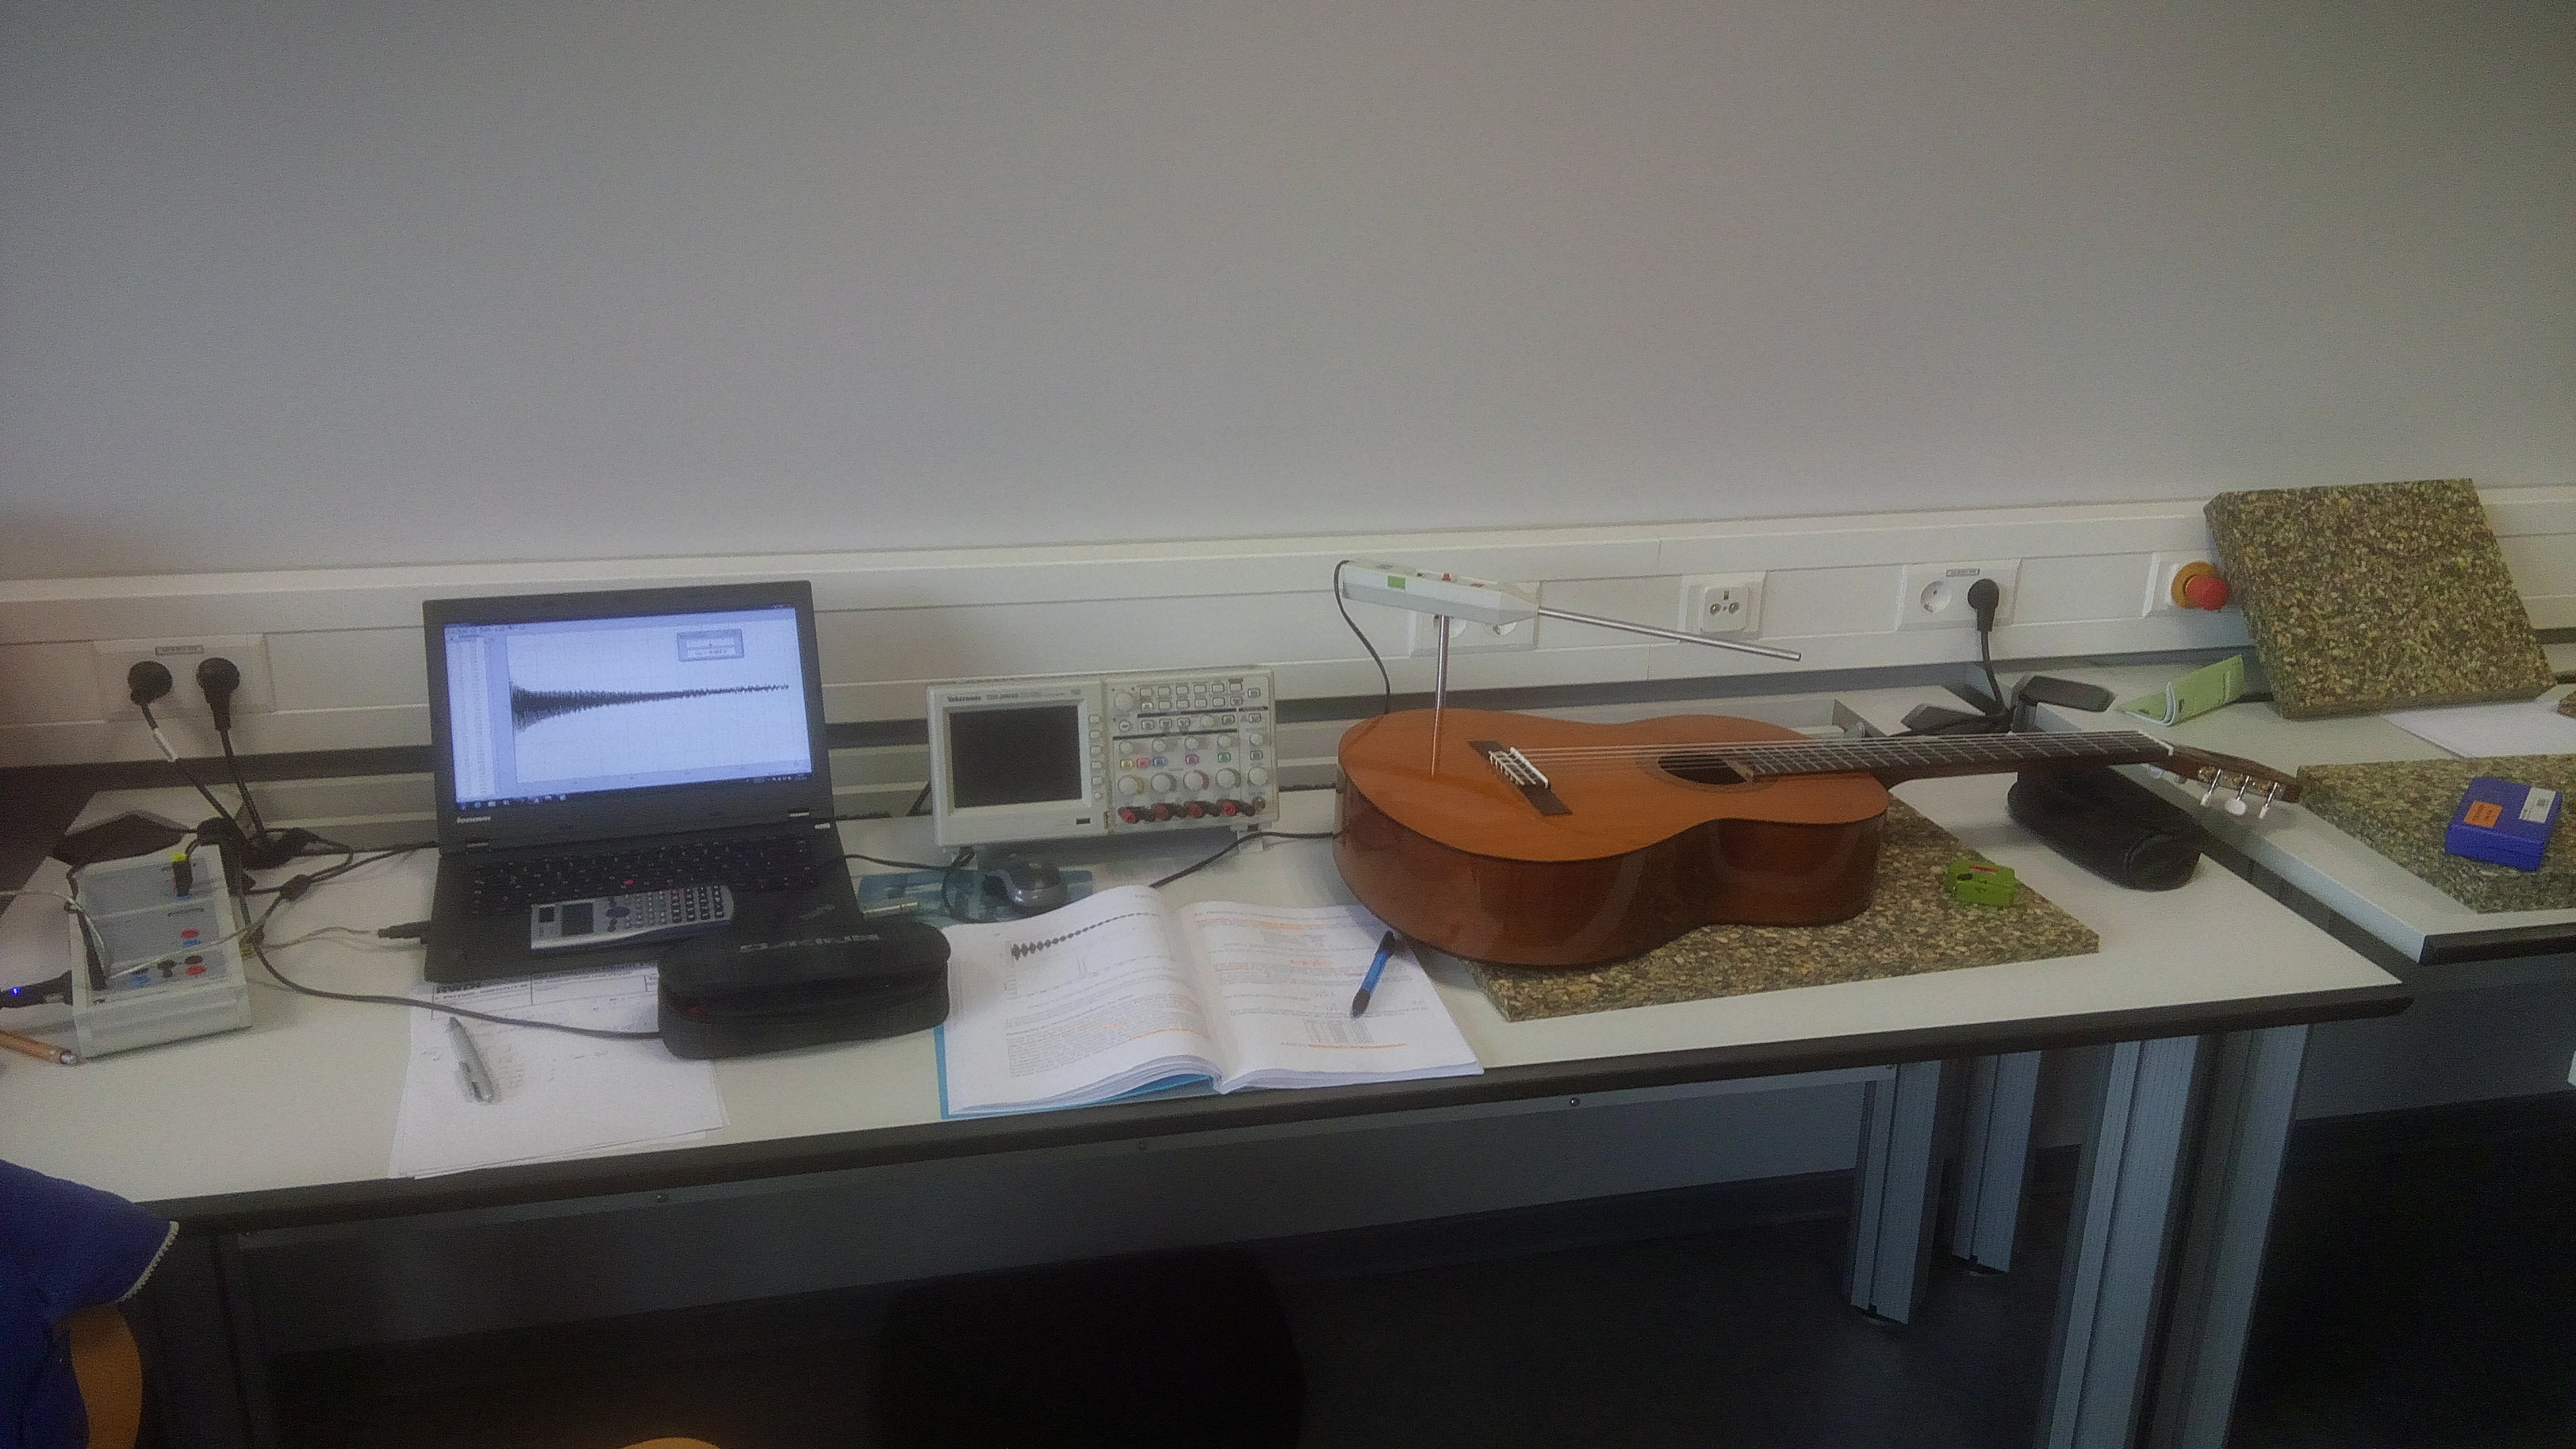
\includegraphics[scale=0.1]{Bilder/IMG_20160323_123920.jpg}
\caption{Versuchsaufbau für Messungen mit der Gitarre. }
\end{figure}


\begin{table}[H]\centering
\caption{Messparameter für Stimmversuche}
\begin{tabular}{c|c}
Parameter & Einstellungen \\ 
\hline
Messintervall & 500 $\mu s$ \\ 
Anzahl Messwerte & 10000 \\ 
Messdauer & 5s \\ 
Trigger & 0.3V \\ 
\end{tabular}
\end{table}
 

Wenn nun die D-Saite leer und die A-Saite im 5. Bund angeschlagen wurde, hörte man denselben Ton ohne Schwebung.

\begin{figure}[H]
\centering
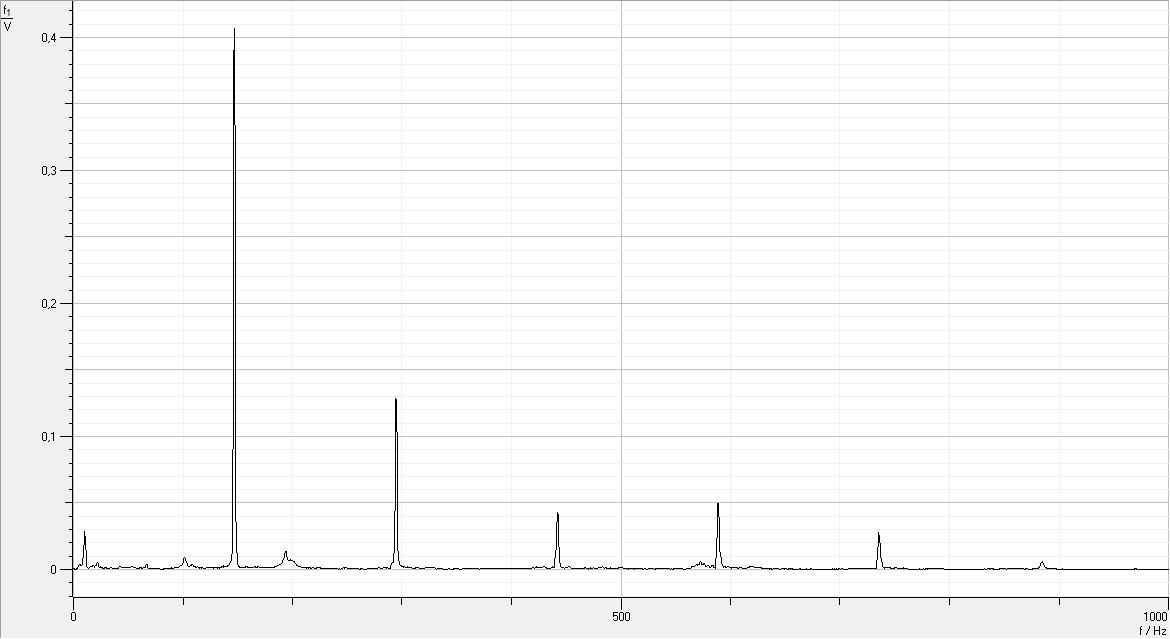
\includegraphics[scale=0.5]{Bilder/Gestimmt_Vorher.png}
\caption{D-Saite leer und A-Saite im 5. Bund nach dem Stimmen mit dem Stimmgerät. Es sind nur jeweils einzelne Peaks sichtbar also keine Schwebung.}
\end{figure}

Als Nächstes wurde die D-Saite so stark verstimmt, dass beim Anschlagen der D-Saite leer und A-Saite im 5. Bund eine deutliche Schwebung zu hören war.

\begin{figure}[H]
\centering
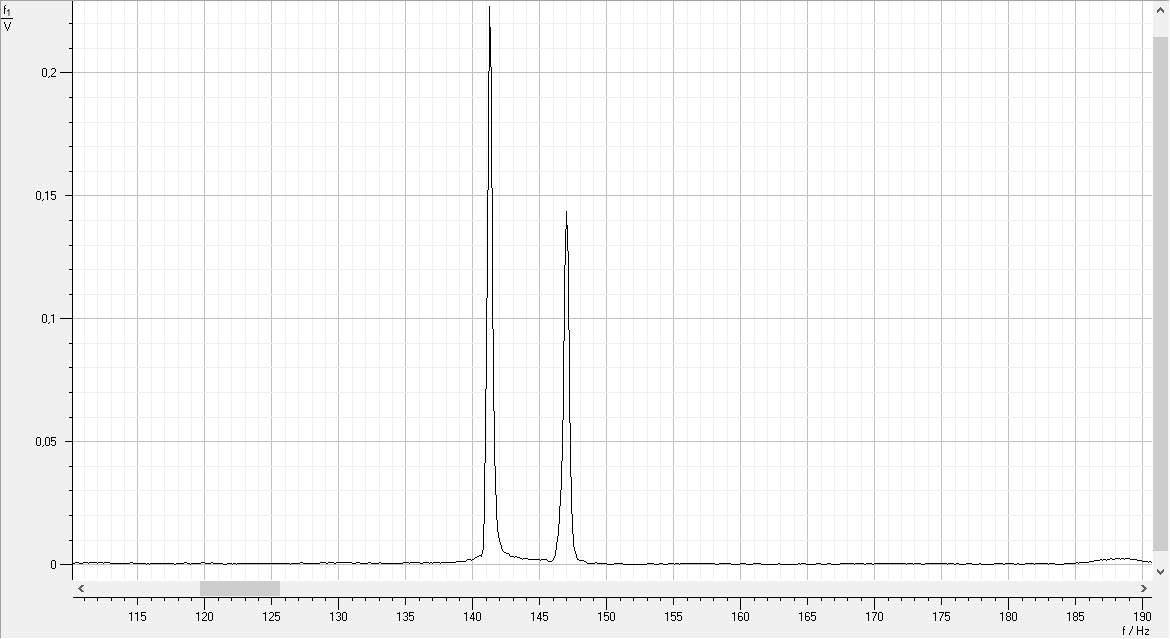
\includegraphics[scale=0.5]{Bilder/Verstimmt.png}
\caption{Verstimmte D-Saite leer und A-Saite im 5. Bund. Es ist eine deutliche Schwebung sichtbar.}
\end{figure}

Die jetzt verstimmte D-Saite wurde daraufhin so weit zurück gedereht bis die Schwebung wieder verschwand.

\begin{figure}[H]
\centering
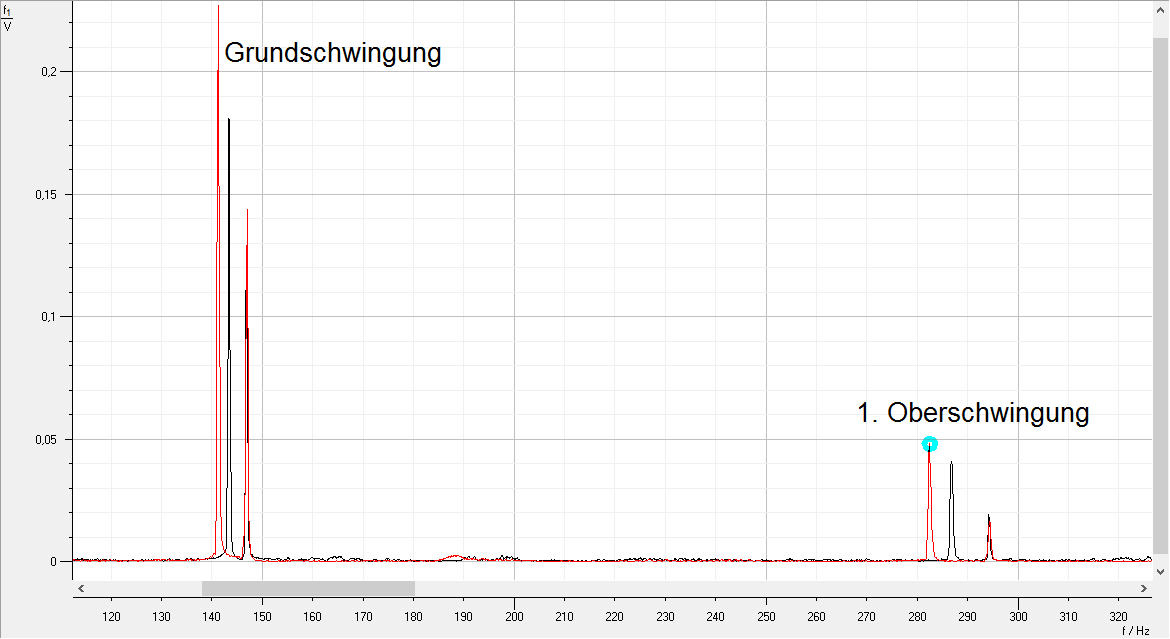
\includegraphics[scale=0.5]{Bilder/Verstimmt_vs_1_stimmen.png}
\caption{Verstimmte D-Saite in rot gegen den ersten Stimmversuch in schwarz. Die Peaks nähern sich. Besonders in der ersten Oberschwingung sieht man die Unterschiede noch deutlicher.}
\end{figure}

\begin{figure}[H]
\centering
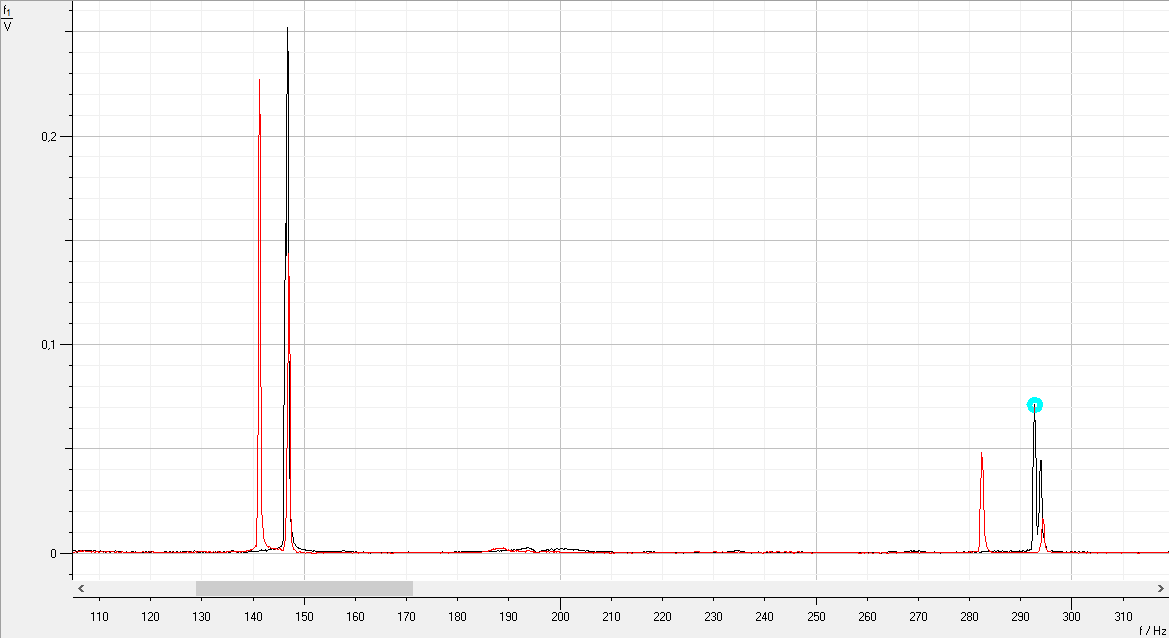
\includegraphics[scale=0.5]{Bilder/Verstimmt_vs_2_stimmen.png}
\caption{Verstimmte D-Saite in rot gegen den zweiten Stimmversuch in schwarz. Bei dem Peak der Grundschwingung ist schon keine Schwebung erkennbar aber in der 1. Oberschwingung sieht man noch eine leichte Schwebung.}
\end{figure}

\begin{figure}[H]
\centering
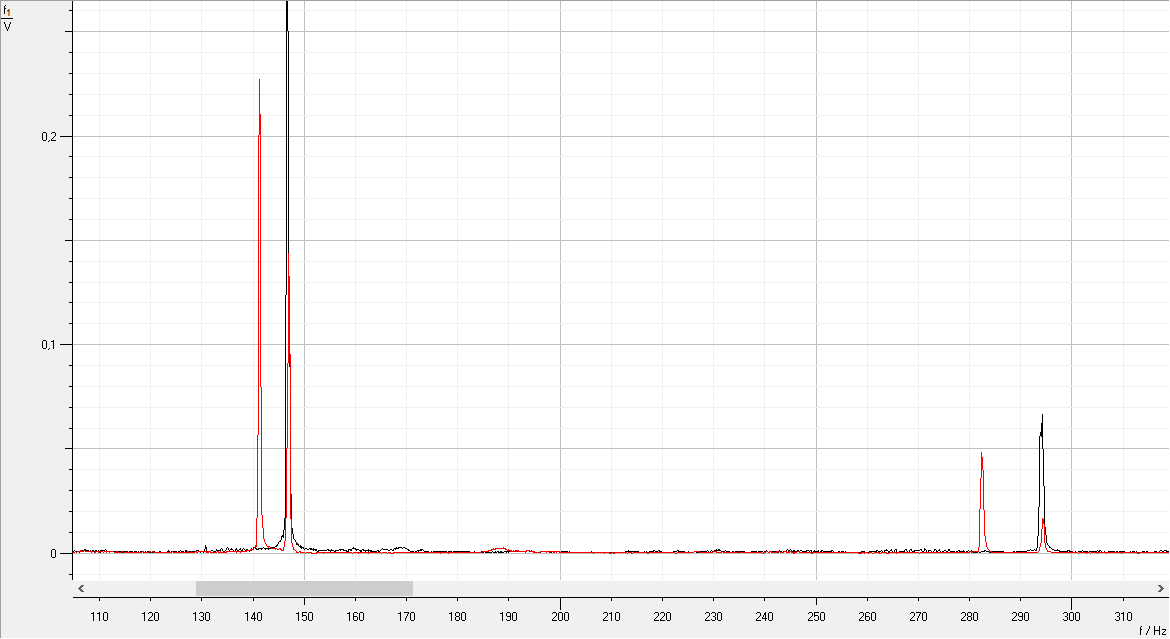
\includegraphics[scale=0.5]{Bilder/Verstimmt_vs_3_stimmen.png}
\caption{Verstimmte D-Saite in rot gegen den dritten Stimmversuch in schwarz. Bei den Peaks der Grundschwingung und der 1. Oberschwingung ist keine Schwebung erkennbar.}
\end{figure}

Die D-Saite sollte nun also wieder gut gestimmt sein, was auch mit dem Stimmgerät überprüft wurde. Das Stimmen über die Schwebung war also erfolgreich.


\end{document}